\section{Satellite System Development}
\label{sec:spaceSystemSimulator}

This section presents the \sss that emulates the real behaviour of a satellite constellation of 17 satellites that download images to a network of 12 ground stations connected with the \bonfire cloud. The simulator is implemented in \vw.

The \sss is constituted of three components:
\begin{itemize}
\item \satss: it simulates the dynamics and communications of the constellation of 17 Earth observation satellites.
\item \gsss: it simulates the dynamics and communications of the network of 12 ground stations distributed around the World.
\item \emph{Distributed Database:} it contains all the required information and parameters to initialize the simulators and make them run in every specific simulator.
While the \satss and the \gsss are implemented in \vw, the distributed database
is computed in the \bonfire cloud.
\end{itemize}

To adapt the \sss to the Fed4FIRE testbeds, some located scenarios were designed in order to reduce the amount of data to process, store and distribute during the simulations. Thus the simulation is shortened to a specific time required to acquire and download certain areas of interest \emph{(AOI)}.

The detailed design of the \sss and its implementation in \vw are next presented.

\subsection{Image Acquisition}
\label{sec:image-acquisition}

The first step is to implement the acquisition of images by the satellites of
the six predefined scenarios (for an extended description on the scenarios see
Anexo~\ref{anexox}) with the satellite
constellation:
%\begin{enumerate}[label=\bfseries Scenario \arabic*:]

\begin{enumerate}
\item Emergencies – Lorca Earthquake (Spain)
\item  Infrastructure monitoring. Affection in railway infrastructures by sand movement in desert areas (Spain)
\item Land Management – South West of England
\item Precision Agriculture – Argentina
\item Basemaps – Worldwide
\end{enumerate}

In each scenario, an Area of Interest \emph{(AOI)} is defined to be acquired
during the simulation. The in orbit satellites are nadir pointing in order to acquire images of the sub satellite point over the Earth surface as shown in Figure \ref{fig:sss-example-strip}.
\begin{figure}[!h]
\begin{center}
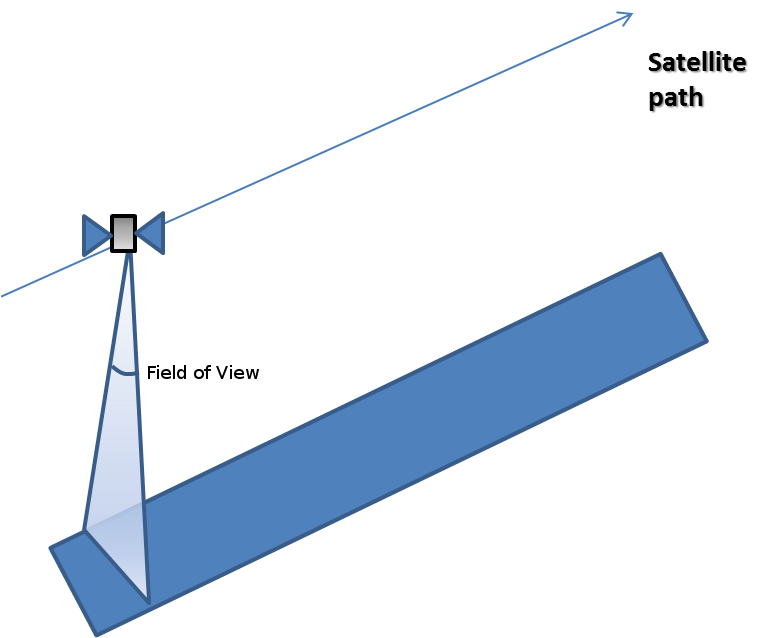
\includegraphics[width=0.6\textwidth]{spaceSystemSimulator/strip-imaging.png}
\caption{Example of strip imaging}
\label{fig:sss-example-strip}
  \end{center}
\end{figure}

In the next subsection the assumptions to simulate the system as realistically
as possible are described for the scenarios. Note that the \emph{AOI} of the scenario 5 is the whole land mass on Earth. This involves that because of the huge amount of data that has to be recorded, specific assumptions to the scenario 5 was made according to the Fed4FIRE testbeds’ limitations.

\subsubsection{Assumptions in satellite image acquisition}
\label{subsubsec:assumptions}

The \emph{AOI} in each scenario can be acquired by one or more satellites depending on
the size of the \emph{AOI} relatively to the scene size (note that the GEO-Cloud
satellites have a swath of $160~km$, thus we divide the acquisition into scenes of
$160~km$ x $160~km$).
In each scenario we call \emph{main satellites} to the satellites with the task
of acquiring the \emph{AOI} (note that all satellites are \emph{main satellites} in the
model for the scenarios 5 and 6).

Along the duration of the scenario other satellites acquire images of the areas
of the Earth surface they are passing over. Those images are not in the area of
interest.

During the experiments in \bonfire, they will be processed but not stored into the system, since the focus of the mission in every scenario has to be in the defined area of interest. Those non \emph{AOI} images allow us to emulate a real system, since we take into account all the possible inputs to the system (note that in the scenarios 5 and 6 all the images created are \emph{AOI}).


\begin{figure}[!h]
\begin{center}
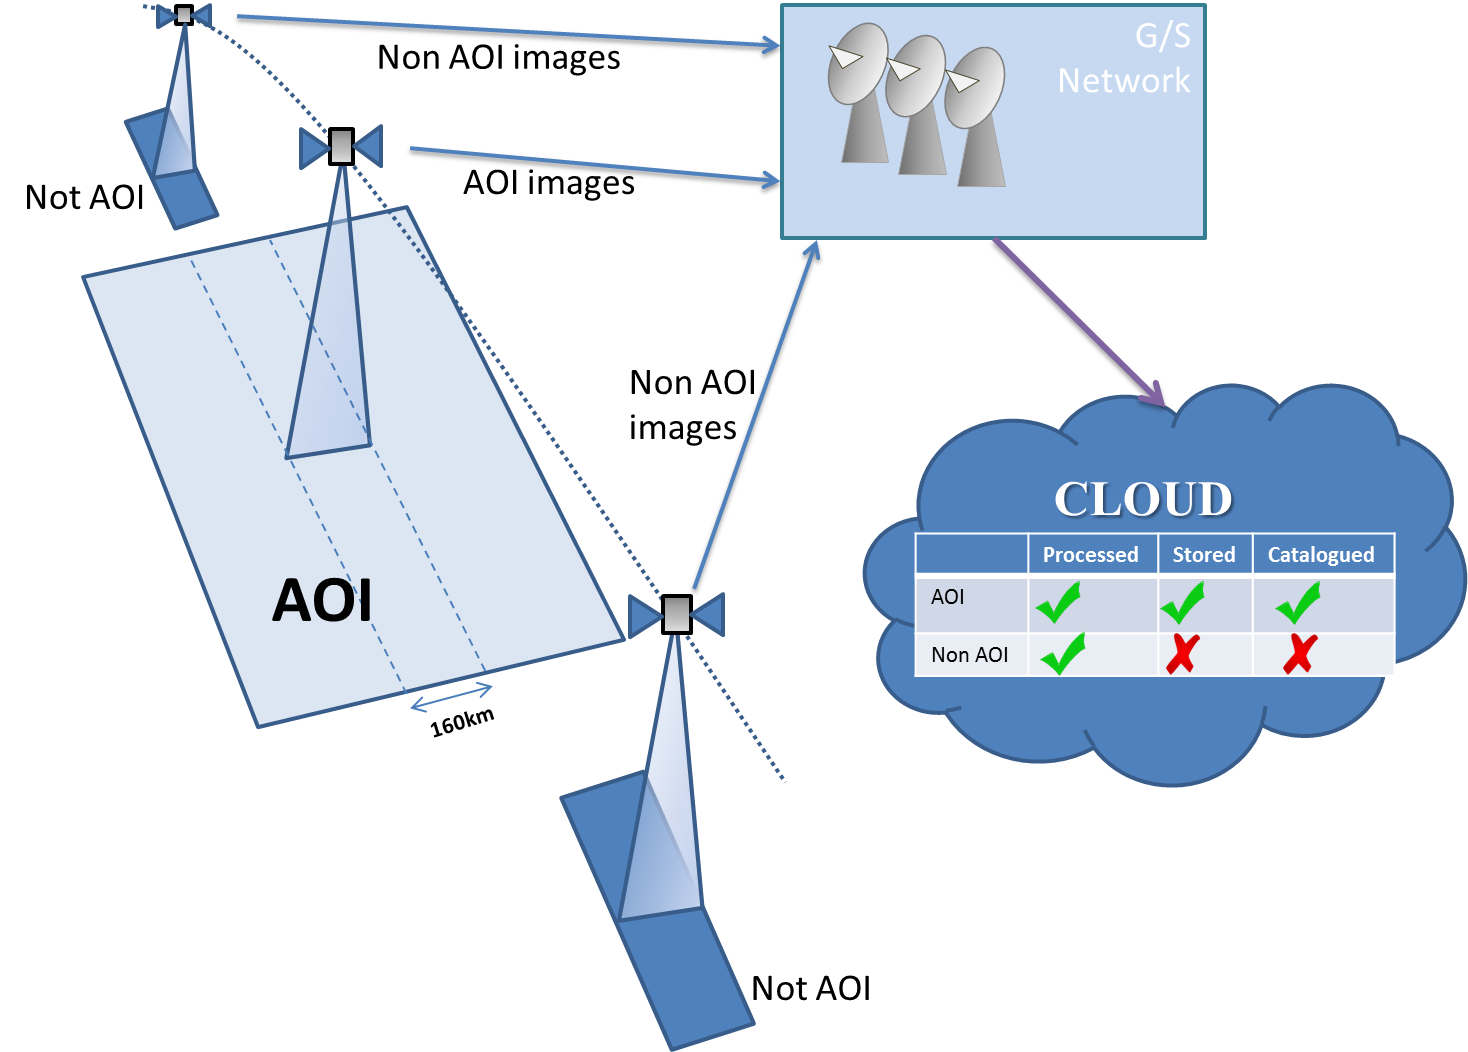
\includegraphics[width=0.8\textwidth]{spaceSystemSimulator/images-adquisition-diagram.png}
\caption{Diagram of images adquisition}
\label{fig:sss-acquisition-diagram}
\end{center}
\end{figure}

Thus, those non \emph{AOI} images, during the simulation will be acquired,
downloaded to the ground stations, transferred to the cloud and processed, but
not stored, neither catalogued. In addition, it has to be taken into account
that the main satellites can also acquire some images out of the \emph{AOI}
during the duration of each scenario. Those acquired images are also considered
non \emph{AOI} images.

In every scenario the time is set to 0 when the simulation starts in the Fed4FIRE environment.

These assumptions are summarized as follows:
\begin{enumerate}
\item Only the scenes acquired by a satellite that include the \emph{AOI} are considered to carry out the complete simulation.
\item Images taken by the satellites that are out of the \emph{AOI} are processed but
  not stored into the system to adjust the experiment execution to the resources
  provided by \bonfire.
\end{enumerate}

\subsubsection{Types of acquisition of the AOI by a single satellite}
\label{subsubsec:types-acquisition}

Depending on the relative sizes of both the \emph{AOI} and the scenes, three different
situations can occur when a single satellite is acquiring images (see Figure~\ref{fig:sss-types-aoi-acquisitions}):
\begin{itemize}
\item Simple acquisition: the \emph{AOI} (at least the part to be imaged by the
  satellite) fits into just one scene.

% \begin{figure}[!h]
% \begin{center}
% 
\includegraphics[width=0.3\textwidth]{spaceSystemSimulator/simple-acquisition.png}
% \caption{Simple acquisition}
% \label{fig:sss-simple-acquisition}
% \end{center}
% \end{figure}
\item Multiple consecutive acquisitions: the \emph{AOI} to be acquired by a satellite
fits in a strip with several scenes.
% \begin{figure}[!h]
% \begin{center}
% 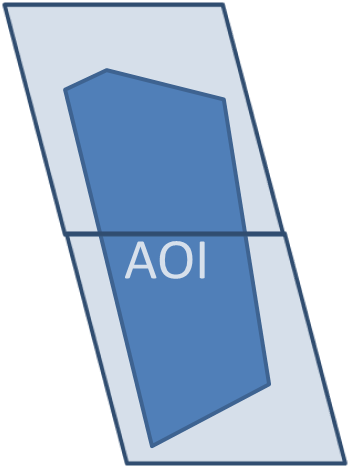
\includegraphics[width=0.3\textwidth]{spaceSystemSimulator/multiple-consecutive-acquisitions.png}
% \caption{Multiple consecutive acquisitions}
% \label{fig:sss-multiple-acquisition-diagram}
% \end{center}
% \end{figure}

\item Multiple non-consecutive acquisitions: the \emph{AOI} to be acquired by a
  satellite fits in a strip but there are some scenes between the acquisitions
  that have to be acquired in order to complete the general mission (world map
  daily) but it is not necessary for the scenario.
\end{itemize}

% \begin{figure}[!h]
% \begin{center}
% 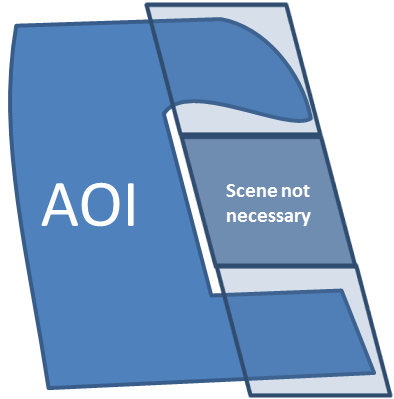
\includegraphics[width=0.3\textwidth]{spaceSystemSimulator/non-consecutive-acquisitions.png}
% \caption{Multiple non-consecutive acquisitions}
% \label{fig:sss-non-consecutive-acquisition}
% \end{center}
% \end{figure}
\begin{figure*}
\begin{center}
  \subfloat[Simple acquisition]{
    
\includegraphics[width=0.25\textwidth]{spaceSystemSimulator/simple-acquisition.png}
    \label{fig:sss-simple-acquisition}
  }
 \hspace{0.01\textwidth}
 \subfloat[Multiple consecutive acquisitions]{
    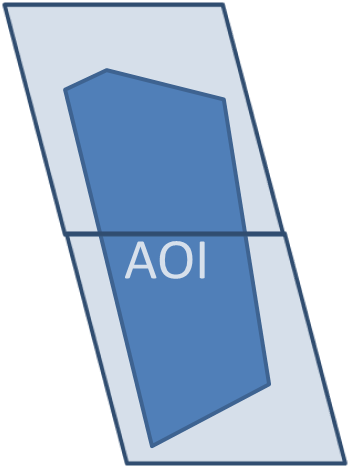
\includegraphics[width=0.25\textwidth]{spaceSystemSimulator/multiple-consecutive-acquisitions.png}
    \label{fig:sss-multiple-consecutive-acquisition}
  }
\hspace{0.01\textwidth}
 \subfloat[Multiple non-consecutive acquisitions]{
    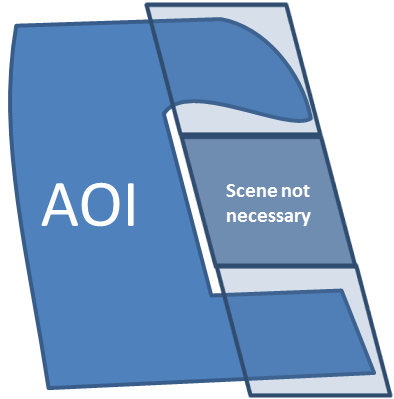
\includegraphics[width=0.25\textwidth]{spaceSystemSimulator/non-consecutive-acquisitions.png}
    \label{fig:sss-non-consecutive-acquisition}
  }
\caption{Different types of the AOI acquisitions}
\label{fig:sss-types-aoi-acquisitions}
\end{center}
\end{figure*}



\subsubsection{Parameters required for the simulation of the scenarios}
\label{subsubsec:parameters-required}
For each scenario, the following parameters and assumptions are considered:
\begin{enumerate}
\item \emph{S: Scenario number.} It indicates the scenario that is being simulated (from 1 to 6).
\item \emph{Main satellites:} The main satellites are those that acquire images of the AOI in each scenario. Notice that all the satellites are numbered from 1 to 17.
\item \emph{ADR:} Acquisition Data Rate. Rate at which the images are acquired
  by the satellite.

\begin{equation} \label{eq:ADR}
ADR=1395~Mbps
\end{equation}

\item \emph{CR:} Compression Rate. Rate at which the images are compressed in
  the satellite for their download.
\begin{equation}\label{eq:CR}
CR=14.1
\end{equation}
\item \emph{$Bandwidth_{sat}$:} Download rate between the satellites and the
  ground stations.
\begin{equation}\label{eq:Bandwidth}
Bandwidth_{sat}=160~Mbps
\end{equation}

The previous bandwidth is used as follows:
\begin{itemize}
\item The satellite is downloading images in memory and at the same time is
  acquiring images and downloading them:
\begin{equation}\label{eq:totalBandwidth}
Bandwidth_{sat}=Bandwidth_{(sim\_acq)}+Bandwidth_{mem}
\end{equation}

where $Bandwidth_{(sim\_acq)}$ is the bandwidth used for downloading images that
are being acquiring at the same time and $Bandwidth_{mem}$ is the bandwidth used
to download images in the satellite memory. $Bandwidth_{(sim\_acq)}$ can be
obtained as follows:
\begin{equation}\label{eq:bandwidth-sim}
  Bandwidth_{(sim\_acq)}=\frac{ADR}{CR}=98.9~Mbps
\end{equation}

where \emph{ADR} is the Acquisition Data Rate (Mbps) and \emph{CR} the data
compression rate. And $Bandwidth_{mem}$ can be obtained as follows:
\begin{equation}\label{eq:bandwidth-mem}
  Bandwidth_{mem}=Bandwidth_{sat}-Bandwidth_{(sim\_acq)}=61.1~Mbps
\end{equation}
\end{itemize}

\item \emph{$T_0$:} Start time. It is the start time of the scenario. The scenario starts when the first main satellite begins the acquisition of the first portion of \emph{AOI}.
\item \emph{$T_f$:} End time. It is the time when the last main satellite finishes the downloading of the \emph{AOI} taken images.
\item \emph{$[T_{AOI}]_{0i}$:} Time a main satellite starts acquiring the \emph{AOI}. $i$ stands for the number of the main satellite.
\item \emph{$[T_{AOI}]_{fi}$:} This is the time a main satellite finishes acquiring a piece of \emph{AOI}.
\item \emph{$[\Delta T_{AOI}]_i$:} This is the difference
  $[T_{AOI}]_{fi}-[T_{AOI}]_{0i}$. Note: Some satellites (all of them in the
  model for scenario 5) can require more than one orbit to acquire the
  corresponding \emph{AOI}, and then these satellites will have a different
  $[\Delta T_{AOI}]_i$ in each acquisition of \emph{AOI}. $[\Delta T_{AOI}]_i$
  is a multiple of  $T_{scene}=23.4~s$, which is the needed time to acquire one
  scene of $160~km$x $160~km$, considering that satellite velocity on ground is
  $v_{Gsat}=6.84~km/s$:
\begin{equation}\label{eq:Tscene}
	T_{scene}=L_{scene}/v_{Gsat}
\end{equation}

$[\Delta T_{AOI}]_i$  can be calculated as follows:
\begin{equation}\label{eq:deltataoi}
[\Delta T_{AOI}]_i=n L_{scene}/v_{Gsat} =nT_{scene}=[T_{AOI}]_{fi}-[T_{AOI}]_{0i}
\end{equation}

where $n$ is the number of scenes, $L_{scene}$  is the length of the scene (in
this case $160~km$), and $v_{Gsat}$ the velocity of the satellite on ground (in this case $6.84~km/s$).
\item \emph{$[T_{GS}]_{0ij}$:} Time a main satellite $i$ enters into the visibility cone of a \emph{Ground Station} $j$.
\item \emph{$[T_{GS}]_{fij}$:} Time a main satellite $i$ leaves the visibility cone of a Ground Station  $j$.
\item \emph{$[\Delta T_{GS}]_{ij}$:} This is the difference $[T_{GS}]_{fij}-[T_{GS}]_{0ij}.$
\item \emph{$T_{start}$:} This is the start time of the simulation. We chose to be $5$ seconds in order to synchronize all the satellites.

\end{enumerate}

As an example, the Table~\ref{table:sss-acquisitions-scenario2} shows the data was obtained from ``Scenario 2: Infrastructure monitoring affection in railway infrastructures by sand movement in desert areas'':

\begin{table}[h]
  \centering
  {\small
  


\begin{tabular}{c c c c c c c}\hline
\tabheadformat
\tabhead{Scenario} & \tabhead{Start Time} &
\tabhead{End Time} & \tabhead{Main} & \tabhead{Start} &
\tabhead{End} &\tabhead{Number of}\\
\tabheadformat
 & $T_0$&$T_f$ &\tabhead{Satellite} & \tabhead{Acquisition}&\tabhead{Acquisition} &\tabhead{\emph{AOI} scenes}\\
 \tabheadformat
 & & & & $[T_{AOI}]_{0i}$&$[T_{AOI}]_{fi}$ & \\\hline
\multirow{3}{*}{2} & \multirow{3}{*}{54060} & \multirow{3}{*}{54753.4}&4 & 54060&54083.4&\multirow{3}{*}{1} \\\cline{4-6}
                   &        &         & 3 & 54390&54413.4 \\\cline{4-6}
                   &        &         & 2 & 54730&54753.4  \\\hline      
\end{tabular}

  }
  \caption{Example of data of image acquisition for Scenario 2}
  \label{table:sss-acquisitions-scenario2}
\end{table}


\subsection{Image Downloading}
\label{subsec:image-downloading}

The acquired images by the satellites shall be downloaded to the emulated ground
stations through the antennas network designed (see Section~\ref{subsec:system-design}). All the scenarios finish at $T_f$, when the last
main satellite completely downloads the last acquired portion of the
\emph{AOI}. During the simulation, the rest of the satellites not overflying the
\emph{AOI} would be imaging other places; these images will also be downloaded
and processed in parallel to the \emph{AOI} images to simulate a realistic case,
but as previously explained those images will not be stored nor catalogued.

Because of the limitations in the testbeds (limited storage and compute
resources in \bonfire cloud and multiplexed channel over virtual networks in
\vw) it is necessary to scale the data involved in these simulations from the
original design of the GEO-Cloud experiment. It has been decided to change the
designed compression rate from lossless compression $2:1$ to a rate compression
$14:1$. With this change, the data volume has been reduced and the size of every
$160km$ x $160km$ scene after compression is now $288~MB$ instead of the almost
$2~GB$ size of the original images.

In order to download the data, the satellites have to be inside the visibility
cone of a ground station. During these accesses, the satellites download images
at a rate of $160~Mbps$. Part of these images are in memory before entering the
visibility cone and others are being acquired simultaneously during the
downloading task (see section \ref{subsubsec:parameters-required} for a wider explanation of the download parameters and Figure \ref{fig:sss-multiplexed-downloading}).

\begin{figure}[!h]
\begin{center}
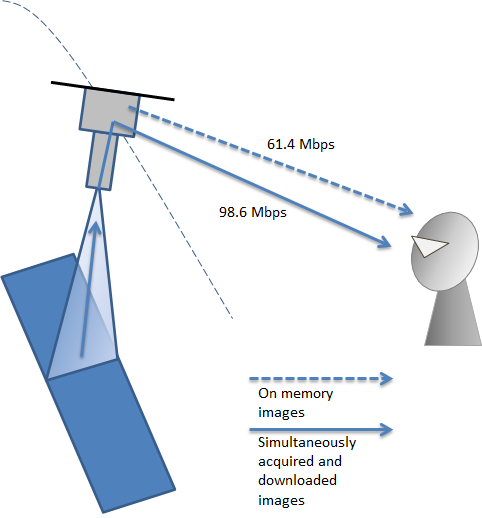
\includegraphics[width=0.5\textwidth]{spaceSystemSimulator/multiplexed-downloading.png}
\caption{Multiplexed images downloading}
\label{fig:sss-multiplexed-downloading}
\end{center}
\end{figure}



It is possible that the duration of the accesses and the time to download an image are not multiples of $T_{scene}=23.4~s$. In this case, an image would be partially downloaded at the end of the access but it would be supposed that this image is completely downloaded in the following access in other ground station.

For the memory management, a \emph{LIFO} (last in, first out) procedure is
applied. This implies that the latest acquired images will be downloaded as soon
as possible. This imposes that when a satellite is inside the visibility cone of
a ground station both the images latest acquired and the images that are being
acquired of the \emph{AOI} will be simultaneously downloaded by multiplexing
them. Note that because of differences between the rate of acquisition and
downloading, and also because of the compression process, the downloading of
images that are being simultaneously acquired do not occupy all the bandwidth of
$160~Mbps$; the portion not occupied is used to download on board storage also
with a \emph{LIFO} process (See section \ref{subsubsec:parameters-required} numbers 3 to 5).


As an example, the data of the accesses for the Scenario 2 are included in Table~\ref{table:sss-accesses-scenario2}.


\begin{table}[h]
  \centering
  {\small
  
\begin{tabular}{p{.2\textwidth}p{.2\textwidth}c c c}\hline
\tabheadformat
\tabhead{Sat. Ident. Number} & \tabhead{Ground Station} &
\tabhead{Access Start Time} & \tabhead{Access Stop Time}
&\tabhead{Duration of the passes}\\
\tabheadformat
 & &$(s)$ &$(s)$ &$(s)$ \\\hline
        1 & Krugersdorp  & 54184.2 &54516 &331.8\\\hline
        2 & Dubai        & 54184.2 &54516 &331.8\\\hline
        2 & Krugersdorp  & 54549.4&54753.4 &204\\\hline
        3 & Dubai        & 54060 &54753.4&204\\\hline
        4 & Dubai        &54060&54337.5&277.5\\\hline              
        4 & Svalvard     &54660&54753.4&93.4\\\hline
        5 & Svalvard     &54316.3&54753.4&437.1\\\hline
        6 & Prince Albert&54708.1&54753.4&45.3\\\hline
        6 & Svalvard     &54060&54639.4&579.4\\\hline
        7 & Prince Albert&54362&54753.4&391.4\\\hline
        7 & Svalvard     &54060&54296.7&236.7\\\hline
        8 & Prince Albert&54060&54577.9&517.9\\\hline
        9 & Prince Albert&54060&54246.8&186.8\\\hline
        15 & Troll       &54419&54670.3&251.3\\\hline
        16 & Troll       &54085.6&54303.4&217.8\\\hline
        17 &Krugersdorp  &54495.4&54753.4&258\\\hline              
\end{tabular}

  }
  \caption{Example of data of accesses for Scenario 2}
  \label{table:sss-accesses-scenario2}
\end{table}


Next, a summary of the assumptions made for the image downloading from the
satellites to the ground stations are described:
\begin{enumerate}
\item Time to process the images on board before downloading is considered to be instantaneous. Then, the simultaneous acquisition and download of the \emph{AOI} inside the visibility cone is done without latency.
\item The ground stations network was designed to guarantee the download of a complete world map in a daily basis. With this assumption into account, the management of the memory on board of each satellite does not require an additional design. This involves that we do not know in which ground station all the areas acquired out of a visibility cone are downloaded.
\item Because of the small gap between the satellites, which are in the same orbit, more than one antenna in each ground station is required to be available. This provides the possibility of having simultaneous contacts with all the satellites inside the visibility cone.
\end{enumerate}

\subsection{Getting the satellite data}
\label{subsec:getting-satellite-data}

The steps to obtain and simulate the realistic behaviour of the satellites are
next described.


\subsubsection{Extraction of the real behaviour of the satellite constellation
  in the scenarios}
\label{subsubsec:extraction}

The first point is to obtain the realistic behaviour of the constellation of satellites designed in section~\ref{subsec:system-design}.  For that purpose, the constellation of satellites and the ground stations were implemented in the \emph{$Systems Tool Kit^{\textregistered}$} (\acs{STK}) software.

The next steps were followed to obtain the values of the parameters required for the simulations of the defined scenarios:
\begin{itemize}
\item Commonly for all the scenarios:
\begin{enumerate}
\item Implementation of the satellite constellation.
\item Implementation of the ground station network.
\item Calculation of the access time for each satellite communicating with each
  ground station during 24 hours.
\newcounter{enumTemp}
\setcounter{enumTemp}{\theenumi}
\end{enumerate}
\item For each different scenario:
\begin{enumerate}
\setcounter{enumi}{\theenumTemp}
\item Identification of the main satellites.
\item Extraction of the times each satellite is acquiring the AOI: $[T_{AOI}]_{0i}$ and $[T_{AOI}]_{fi}$.
\item Calculation of the number of scenes acquired: $n$.
\item Extraction of the access duration of each satellite with the ground stations it communicates within the scenario duration: $[T_{GS}]_{0ij}$ and $[T_{GS}]_{fij}$.
\item Start time of the scenario: $T_0$.
\item End time of the scenario: $T_f$.
\end{enumerate}
\end{itemize}

\subsubsection{Exportation of data to the simulator}

Once obtained the previous data, it is exported to different \ac{CSV} format files:

\begin{itemize}
\item 	The \emph{Scenario\_<NUM>\_<SCENE>.csv} files: it contains the information
  of the $[T_{GS}]_{0ij}$ and $[T_{GS}]_{fij}$ for each scenario. \emph{<NUM>} indicates
  the number of the scenario and \emph{<SCENE>} the name of the scenario. In the
  GEO-Cloud experiment we simulate 6 scenarios. The previous parameters are
  defined in the following table:


For example, the format of the resulting \emph{Scenario\_1\_
Emergencies\_Lorca\_Earthquake.csv} file with the $[T_{GS}]_{0ij}$ and $[T_{GS}]_{fij}$
information for the Lorca scenario, looks like the code extract shown in Listing
\ref{code:sss-info-scenario}.
\begin{listing}[
  float=h!,
  caption  = {Extract of the \emph{Scenario\_1\_Emergencies\_Lorca\_Earthquake.csv}
    of the Lorca scenario},
  label    = code:sss-info-scenario,
style=customc]
"GEO-Cloud_005-To-Troll - Access","Start Time (EpSec)","Start Time (UTCG)","Stop Time (EpSec)","Stop Time (UTCG)","Duration (sec)"
1,63638.000,11 Aug 2014 10:10:38.000,63661.400,11 Aug 2014 10:11:01.400,23.400

"GEO-Cloud_006-To-Troll - Access","Start Time (EpSec)","Start Time (UTCG)","Stop Time (EpSec)","Stop Time (UTCG)","Duration (sec)"
7,63638.000,11 Aug 2014 10:10:38.000,63661.400,11 Aug 2014 10:11:01

\end{listing}
In the code, a heading is separated into columns. It is divided as the
table~\ref{table:sss-headings-scenario2} shows.

\item 	The \emph{All\_Scenarios.csv} file: it contains the information of the $[T_{AOI}]_{0i}$ and $[T_{AOI}]_{fi}$ for all the scenarios.
A piece of the \emph{All\_Scenarios.csv} file that contains the $[T_{AOI}]_{0i}$
and $[T_{AOI}]_{fi}$ of all the scenarios is shown in Listing~\ref{code:sss-all-scenarios}.  It also contains  $T_0$ ,$T_f$ and the number $n$ of \emph{AOI} obtained images.


\begin{listing}[
  float=h!,
  caption  = {Extract of the \emph{All\_Scenarios.csv} code of the Lorca scenario},
  label    = code:sss-all-scenarios,
style=customc]
Scenario,Start Sce,End Sce,Sat,Start sat,End Sat,Images
1,63638,63661.4,11,63638,63661.4,1
,,,,,,
2,54060,54753.4,4,54060,54083.4,1
,,,3,54390,54413.4,1
,,,2,54730,54753.4,1
,,,,,,
3,62480,63865.4,15,62480,62503.4,1
,,,14,62821,62844.4,1
,,,13,63161,63184.4,1
,,,12,63501,63524.4,1
,,,11,63842,63865.4,1
\end{listing}

This file was manually computed. The required fields to describe the behaviour
of the satellites acquiring the \emph{AOI} are the depicted in Table~\ref{table:sss-all-scenarios}.

%\begin{multicols}{2}
%\begin{center}
\begin{table}[h]
  \centering
  {\small
  


\begin{tabular}{p{.2\textwidth}p{.2\textwidth}}
  \tabheadformat
  \tabhead{Column Title}   &
  \tabhead{Function}\\
\hline
\textit{GEO-Cloud\_sat-To-station}         & Represents the access of a satellite to the specific ground station. sat represents the satellite number and station the ground station name. \\
\hline
\textit{Start Time (EpSec)}         & Means $[T_{GS}]_{0ij}$. \\
\hline
\textit{Start Time (UTCG)}         & Means  $[T_{GS}]_{0ij}$ in UTCG format \\
\hline
\textit{Stop Time (EpSec)}         & Means $[T_{GS}]_{fij}$ \\
\hline
\textit{Stop Time (UTCG)}         & Means $[T_{GS}]_{fij}$ in UTCG format. \\
\hline
\textit{Duration (sec)}         & Means $[\Delta T_{GS}]_{ij}$. \\
\hline
\end{tabular}


% Local variables:
%   coding: utf-8
%   ispell-local-dictionary: "castellano8"
%   TeX-master: "main.tex"
% End:

  }
  \caption{Columns headings \emph{Scenario\_<NUM>\_<SCENE>.csv} files}
  \label{table:sss-headings-scenario2}
\end{table}
%\end{center}

%\columnbreak
%\begin{center}
\begin{table}[h]
  \centering
  {\small
  


\begin{tabular}{p{.2\textwidth}p{.2\textwidth}}
  \tabheadformat
  \tabhead{Column Title}   &
  \tabhead{Function}\\
\hline
\textit{Scenario}         & Scenario number. Indicates the scenario executed \\
\hline
\textit{Start Sce}         & Indicates the start of the scenario. It is $T_0$  \\
\hline
\textit{End Scen}         &Indicates when the scenario finishes. It is $T_f$ \\
\hline
\textit{Sat}         & Indicates the number of the \emph{main satellite}.\\
\hline
\textit{Star Sat}         & The time when the satellite starts acquiring the \emph{AOI}. It is $[T_{AOI}]_{0i}$. \\
\hline
\textit{End Sat}         & The time when the satellite finishes acquiring the \emph{AOI}. It is $[T_{AOI}]_{fi}$ \\
\hline
\textit{Images}         & This is the number of \emph{AOI} images. It is $n$.\\
\hline
\end{tabular}


% Local variables:
%   coding: utf-8
%   ispell-local-dictionary: "castellano8"
%   TeX-master: "main.tex"
% End:

  }
  \caption{Columns headings of the \emph{All\_Scenarios.csv} file}
  \label{table:sss-all-scenarios}
\end{table}
%\end{center}
%\end{multicols}
\end{itemize}


\subsubsection{Processing of the Scenario\_<NUM>\_<SCENE>.csv and
 All\_Scenarios.csv}
\label{subsubsec:processing-files}

A script is designed and developed to get and merge the data from the \emph{Scenario\_<NUM>\_<SCENE>.csv} and the \emph{All\_Scenarios.csv} files, and to store the information in the database:  \emph{setDatabase.py}. It was developed in Python 2.7 but it is also compatible with all Python versions.

This has to be done because as previously explained
\emph{Scenario\_<NUM>\_<SCENE>.csv} contains the $[T_{GS}]_{0ij}$ and $[T_{GS}]_{fij}$
parameters of each single scenario and \emph{All\_Scenarios.csv} the
$[T_{AOI}]_{0i}$ and $[T_{AOI}]_{fi}$ of all the scenarios. Thus the script matches the
$[T_{GS}]_{0ij}$ and $[T_{GS}]_{fij}$ of one scenario with the $[T_{AOI}]_{0i}$ and $[T_{AOI}]_{fi}$ of such a scenario.

To execute \emph{setDatabase.py} the arguments depicted in Table~\ref{table:sss-arguments-setdatabase} are required.
\begin{table}[h]
  \centering
  {\small
  


\begin{tabular}{p{.2\textwidth}p{.2\textwidth}}
  \tabheadformat
  \tabhead{Argument Position}   &
  \tabhead{Meaning}\\
\hline
\textit{1}         & IP direction of the host which contains the MySQL database\\
\hline
\textit{2}         & The relative path or absolute path of the file that contains the information of all scenarios (see Listing \ref{code:sss-all-scenarios})
  \\
\hline
\textit{3\ldots}         &The \emph{Scenario\_<NUM>\_<SCENE>.csv} files that contain the events occurred in a particular scenario. At least one file must be introduced, otherwise an execution error is produced. \\\hline
\end{tabular}


% Local variables:
%   coding: utf-8
%   ispell-local-dictionary: "castellano8"
%   TeX-master: "main.tex"
% End:

  }
  \caption{Arguments of \emph{setDatabase.py}}
  \label{table:sss-arguments-setdatabase}
\end{table}

An example of the execution of the programme is the following:
\begin{itemize}
\item[>] python~setDatabase.py~192.168.0.2~All\_scenarios\_file.csv~Scenario\_1\_Example1.csv~Scenario\_2\_Example2.csv~Scenario\_3\_Example3.csv
\end{itemize}


\subsection{Space System Simulator}

The \sss is constituted by the following modules:
\begin{itemize}
\item The Database
\item The \satss
\item The \gsss
\end{itemize}


To simulate every scenario, on the one hand, the \satss is executed. It is
constituted by 17 \emph{Satellite Simulators} of individual satellites; each one
reproduces the characteristic behaviour of every single satellite in the
constellation.
On the other hand the \gsss is also executed. As in the case of the \satss, the
\gsss is constituted of 12 \emph{Ground Station Simulators} of individual ground
stations reproducing the behaviour of every single ground station of the
designed network.

The diagram in Figure~\ref{fig:sss-architecture} depicts a scheme
representing the \emph{Space System Simulator}.

\begin{figure}[!h]
\begin{center}
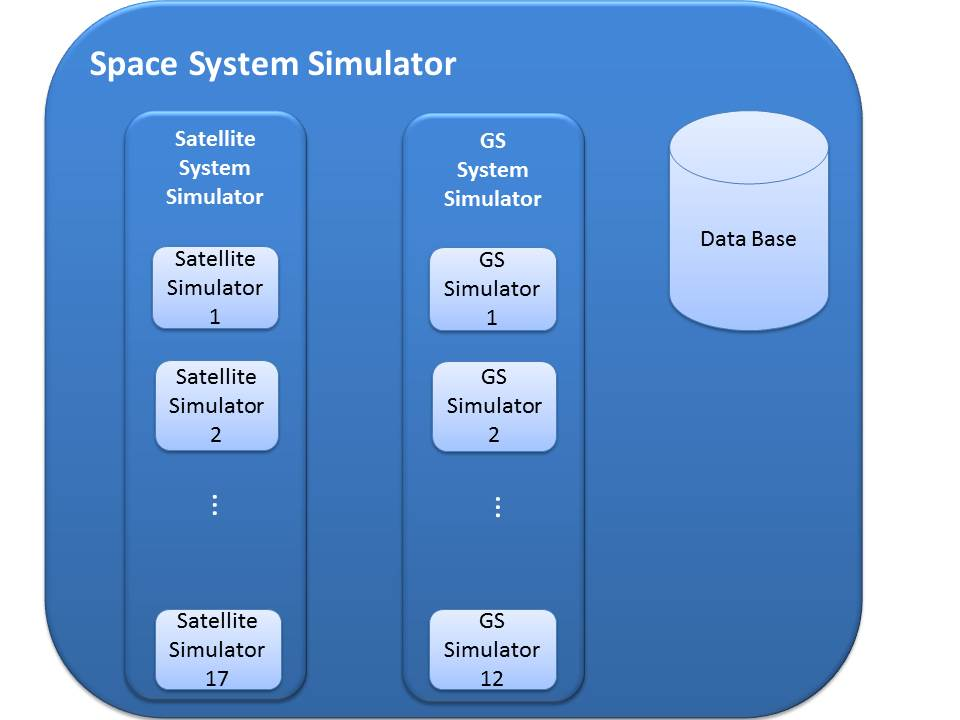
\includegraphics[width=0.8\textwidth]{spaceSystemSimulator/sss-architecture.jpg}
\caption{Space System Simulator's Architecture}
\label{fig:sss-architecture}
\end{center}
\end{figure}

The Space System Simulator sequentially follows the next steps during the
execution:
\begin{itemize}

\item First, \emph{setDatabase.py} is executed. The script fills the database fields with the information of every scenario.
\item Second, the \gsss is executed. The \gsss can execute all the \emph{Ground Station Simulators} or some of them individually to simulate faults in the ground stations as it can occur in reality. Thus, when a satellite needs to download data into a ground station that is offline, it will receive an exception so the downloading of images does not start.
\item Third, the \satss is executed. As in the previous case, the \satss can execute all the \emph{Satellites Simulators} or some of them individually for the same reason.
\item Finally, when the scenario finishes, the simulation is stopped.
\end{itemize}
The \emph{Database}, the \satss and the \gsss are thoroughly described in the
next subsections.

\subsubsection{Database}

A database containing all the required data for the simulations was
implemented. The selected database management system \emph{(DBMS)} is
\emph{MySQL}. It was selected because it is friendly usable, works in multiple
platforms, provides transactional and nontransactional storage engines and the server is a separate program for use in a \emph{client/server} networked environment.

The design of the database architecture is shown in Figure~\ref{fig:sss-database-architecture}.

\begin{figure}[!h]
\begin{center}
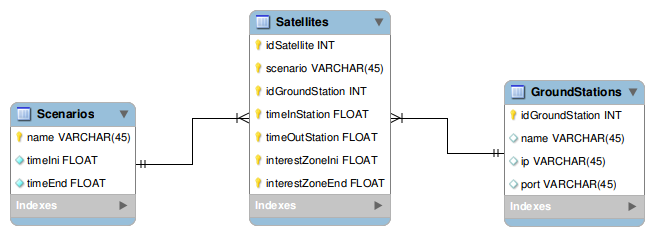
\includegraphics[width=0.85\textwidth]{spaceSystemSimulator/database-architecture.png}
\caption{Database architecture}
\label{fig:sss-database-architecture}
\end{center}
\end{figure}

The database is constituted by three tables: \emph{Scenarios table},
\emph{Satellites table} and \emph{GroundStations table}. The functionalities of the tables are described in
Table~\ref{table:sss-funcionalities-database}.

% \begin{table}[h]
%   \centering
%   {\small
%   


\begin{tabular}{p{.2\textwidth}p{.2\textwidth}p{.2\textwidth}p{.2\textwidth}}
  \tabheadformat
  \tabhead{Table}   & \tabhead{Function}& \tabhead{Columns} &
  \tabhead{Relationship}\\\hline

\textit{Scenarios table}    &  It contains the name of the scenario, the start
time $T_0$ and the end time $T_f$. Its primary key\footnote{The \emph{primary
    key} identifies an object; for example a scenario, a ground station or a
  satellite} (represented with a key symbol in
Figure~\ref{fig:sss-database-architecture}) is the name column.   & name timeIni
timeEnd&None\\
\hline


\textit{GroundStations table} & It contains the ID of the Ground Station and its
name. Its \emph{primary key} is the idGroundStation. &
idSatellite scenario idGroundStation timeInStation timeOutStation
interestZoneIni interestZoneEnd
&None  \\\hline

\textit{Satellites table} &  It contains the ID of the satellites
\emph{idSatellite}, the scenario and the ground station id,
\emph{idGroundStation}, in which the events occur, the time in which the
satellite enters into the visibility cone $[T_{GS}]_{0ij}$,
\emph{timeInStation}, the time when it leaves the visibility cone
$[T_{GS}]_{fij}$, \emph{timeOutStation}, the time when the satellite enters into
the \emph{AIO} $[T_{AOI}]_{0i}$, \emph{interestZoneIni}, and the time when the
satellite leaves the \emph{AOI} $[T_{AOI}]_{fi}$,\emph{interestZoneEnd}. All of
them are primary keys because a satellite can download images of several
\emph{AOIs} in a single ground station.
  & idGroundStation name ip port & This table relates the \emph{Scenarios} table and the \emph{GroundStations} table. This is because the \emph{scenario} and \emph{idGroundStation} columns are foreign keys\footnote{The \emph{foreign key} binds two tables, linked across a field. For example in this case, the column from the \emph{Satellites} table which is named \emph{Scenario} refers to an object that exists in the \emph{Scenarios} table.}. The characteristics of these columns are \emph{On delete cascade} and \emph{On update cascade}. This means that when an object contained in a table (\emph{GroundStation} table or \emph{Scenarios} table) is deleted, it is also automatically deleted the object that refers to it, and if it is updated the object is also automatically updated. \\\hline
\end{tabular}


% Local variables:
%   coding: utf-8
%   ispell-local-dictionary: "castellano8"
%   TeX-master: "main.tex"
% End:

%   }
%   \caption{Funcionalities of the database tables for the simulator}
%   \label{table:sss-funcionalities-database}
% \end{table}
 


\begin{tabular}{p{.2\textwidth}p{.2\textwidth}p{.2\textwidth}p{.2\textwidth}}
  \tabheadformat
  \tabhead{Table}   & \tabhead{Function}& \tabhead{Columns} &
  \tabhead{Relationship}\\\hline

\textit{Scenarios table}    &  It contains the name of the scenario, the start
time $T_0$ and the end time $T_f$. Its primary key\footnote{The \emph{primary
    key} identifies an object; for example a scenario, a ground station or a
  satellite} (represented with a key symbol in
Figure~\ref{fig:sss-database-architecture}) is the name column.   & name timeIni
timeEnd&None\\
\hline


\textit{GroundStations table} & It contains the ID of the Ground Station and its
name. Its \emph{primary key} is the idGroundStation. &
idSatellite scenario idGroundStation timeInStation timeOutStation
interestZoneIni interestZoneEnd
&None  \\\hline

\textit{Satellites table} &  It contains the ID of the satellites
\emph{idSatellite}, the scenario and the ground station id,
\emph{idGroundStation}, in which the events occur, the time in which the
satellite enters into the visibility cone $[T_{GS}]_{0ij}$,
\emph{timeInStation}, the time when it leaves the visibility cone
$[T_{GS}]_{fij}$, \emph{timeOutStation}, the time when the satellite enters into
the \emph{AIO} $[T_{AOI}]_{0i}$, \emph{interestZoneIni}, and the time when the
satellite leaves the \emph{AOI} $[T_{AOI}]_{fi}$,\emph{interestZoneEnd}. All of
them are primary keys because a satellite can download images of several
\emph{AOIs} in a single ground station.
  & idGroundStation name ip port & This table relates the \emph{Scenarios} table and the \emph{GroundStations} table. This is because the \emph{scenario} and \emph{idGroundStation} columns are foreign keys\footnote{The \emph{foreign key} binds two tables, linked across a field. For example in this case, the column from the \emph{Satellites} table which is named \emph{Scenario} refers to an object that exists in the \emph{Scenarios} table.}. The characteristics of these columns are \emph{On delete cascade} and \emph{On update cascade}. This means that when an object contained in a table (\emph{GroundStation} table or \emph{Scenarios} table) is deleted, it is also automatically deleted the object that refers to it, and if it is updated the object is also automatically updated. \\\hline
\end{tabular}


% Local variables:
%   coding: utf-8
%   ispell-local-dictionary: "castellano8"
%   TeX-master: "main.tex"
% End:


\subsubsection{Database Filling}

\begin{itemize}

\item \textbf{Filling during initialization}

The database is filled during the initialization process by executing
\emph{setDatabase.py} as previously described in section~\ref{subsubsec:processing-files}. This execution makes the following sequential
actions:
\begin{enumerate}
\item All the data that is in the database is cleaned to avoid inconsistencies.
\item The \emph{GroundStation} table is filled with the ground stations information (only name and id).
\item The Scenario table is completely filled with the data of each scenario.
\item Finally, the Satellites table is completely filled. This process joins the
  information contained in the \emph{Scenario\_<NUM>\_<SCENE>.csv} with file
  \emph{All\_Scenarios.csv}. This means that for each Scenario the $[T_{GS}]_{0ij}$,
  $[T_{GS}]_{fij}$,  $[T_{AOI}]_{0i}$ and $[T_{AOI}]_{fi}$ representative of the simulated
  scenario are taken. That information is inserted into the database as follows:
\begin{itemize}
\item For each scenario the information regarding the accesses of the satellites to the ground stations are selected, $[T_{GS}]_{0ij}$ and $[T_{GS}]_{fij}$.
\item Those accesses are merged with the \emph{All\_scenarios.csv} file in order to obtain the accesses of the satellites in which there are \emph{AOI} images.
\item Then if the satellite acquired an \emph{AOI} in the current scenario, the information of the \emph{AOI} is also included in the database.
\item Otherwise the fields with the information regarding the \emph{AOI} are filled
  with $-1$ value.
\end{itemize}
\end{enumerate}

\item \textbf{Filling during the execution of the Space System Simulator}

During the execution of the \gsss the ip and port columns in the
\emph{GroundStations} table are filled. This is done when a \emph{Ground Station
  Simulator} starts its execution in a node. The \emph{IP address} and
\emph{port} of that node are obtained and included in the database. Once each
ground station has an \emph{IP address} and a \emph{port} associated, the \emph{Satellite Simulators} can read both of them and communicate with \emph{Ground Stations Simulators} servers.

\end{itemize}


\subsection{Satellite System Simulator}

The \satss reproduces the behaviour of the 17 satellites constellation by executing 17 individual \emph{Satellite Simulators} characterized by the specific behaviour of each satellite.

The \satss is a manager that executes 17 \emph{Satellite Simulators}. The
\emph{Satellite System Simulator} requires the scenario number and the \emph{IP
  adress} of the database as an input and executes the \emph{Satellite
  Simulators} by providing them the specific identity of the satellite
\emph{(idSatellite)}, number of the scenario \emph{(S)} and IP address of the distributed database  \emph{(ipDatabase)}.

Next, the architecture of the \emph{Satellite Simulator} for each individual
satellite is described.


\subsubsection{Satellite Simulator}

The \emph{Satellite Simulator} is constituted by the following components:
\begin{itemize}
\item \emph{Initialization Module:} This module obtains the following parameters
  and initializes the Satellite Simulator:
\begin{itemize}
\item \emph{S:} the number of the scenario to simulate.
\item \emph{idSatellite:} identification number of the satellite (1 to 17).
\item \emph{ipDatabase:} \emph{IP address} of the database.
\end{itemize}
Once obtained the previous parameters, the Initialization Module connects with the database and fetches the $[T_{GS}]_{0ij}$, $[T_{GS}]_{fij}$,  $[T_{AOI}]_{0i}$, $[T_{AOI}]_{fi}$, the \emph{IP addresses} of the \emph{Ground Station Simulators} servers “ipGroundStations” and  the ports of the \emph{Ground Station Simulators} servers “portGroundStations” for the simulated satellite in the specific scenario. Those times$[T_{GS}]_{0ij}$, $[T_{GS}]_{fij}$, $[T_{AOI}]_{0i}$, $[T_{AOI}]_{fi}$ are provided to the \emph{Satellite Dynamics Module}.

\item \emph{Satellite Dynamics Module:} This module represents the dynamics and
  associated parameters of the satellite. It requires $[T_{GS}]_{0ij}$, $[T_{GS}]_{fij}$,  $[T_{AOI}]_{0i}$ and $[T_{AOI}]_{fi}$ of every scenario as inputs, and it provides the acquired images by the satellite in function of the time acquisition (those images are downloaded to the ground stations, simulated by the \gsss).
Figure~\ref{fig:sss-sat-simulator-architecture} shows the relation between the previous modules.
\end{itemize}

\begin{figure}[!h]
\begin{center}
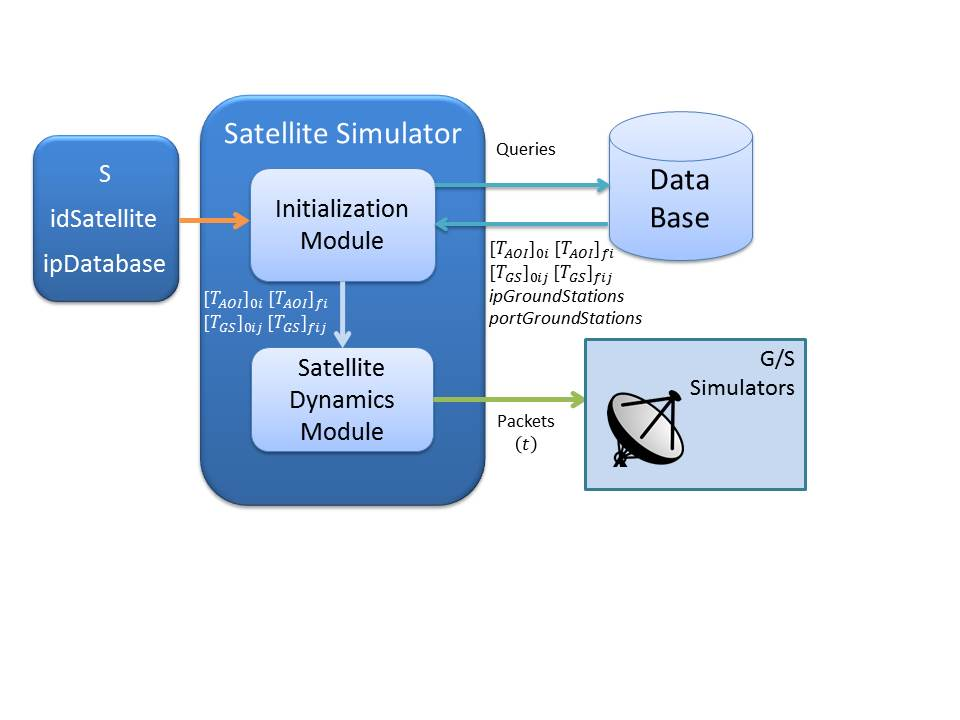
\includegraphics[width=0.7\textwidth]{spaceSystemSimulator/sat-simulator-architecture.jpg}
\caption{Satellite Simulator Architecture}
\label{fig:sss-sat-simulator-architecture}
\end{center}
\end{figure}

\paragraph{Satellite Simulator Workflow}~\\
\label{par:satellite-workflow}
The \emph{Satellite Simulator} starts the execution following these steps:
\begin{enumerate}
\item The \emph{Initialization Module} obtains \emph{S}, \emph{idSatellite} and \emph{ipDatabase}.
\item Then, the \emph{Initialization Module} makes queries on the database to obtain all the required satellite data for current scenario: $[T_{GS}]_{0ij}$, $[T_{GS}]_{fij}$,  $[T_{AOI}]_{0i}$ and $[T_{AOI}]_{fi}$. The queries made to the database contain the particle “order by timeInZone” column. This means that the database returns the $[T_{GS}]_{0ij}$ times in ascending order. Other query gets the \emph{ipGroundStations} and \emph{portGroundStations} of every \emph{Ground Station Simulator}.
\item Schedule of data download: the \emph{Satellite Simulator} schedules the data download from the \emph{Satellite Simulator} to the \emph{Ground Station Simulators} (see Section~\ref{subpar:shedule-process}).
\item When all the communications between the \emph{Satellite Simulator} and the \emph{Ground Station Simulators} have been scheduled in time, the \emph{Satellite Simulator} starts \emph{Satellite Dynamics Module}.
\item When the last scheduled task has been executed, the \emph{Satellite
    Simulator} finishes the execution.
\end{enumerate}
Figure~\ref{fig:sss-sat-simulator-workflow} shows the process explained above. The diagram also shows the
interactions with the other subsystems (see also Figure~\ref{fig:sss-sat-simulator-architecture}). Figure~\ref{fig:sss-sat-simulator-workflow} also shows the inputs for the \emph{Satellite Simulator} and the outputs after its execution. These outputs are the packets in time sent to the ground stations and a log file that contains the information about the execution. In orange the inputs to the \emph{Satellite Simulator} are represented, in green the transitions in the workflow and in blue the outputs.

\begin{figure}[!h]
\begin{center}
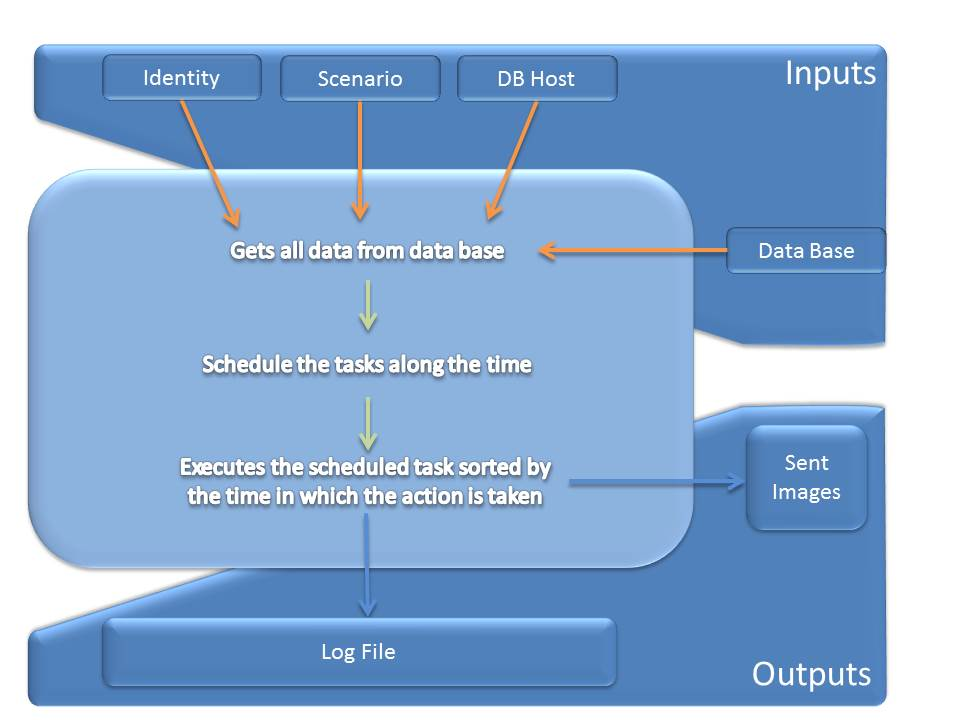
\includegraphics[width=0.8\textwidth]{spaceSystemSimulator/sat-simulator-workflow.jpg}
\caption{Satellite Simulator Workflow}
\label{fig:sss-sat-simulator-workflow}
\end{center}
\end{figure}

\subparagraph{Schedule of data download process}~\\
\label{subpar:shedule-process}
\textbf{Definitions:}

Regarding the images download process, the satellites should download at
$160~Kbps$ to the ground station. In \vw we have a limited bandwidth at
$100~Kbps$. To solve this problem we designed several types of packets (with one
byte size), which are sent between \vw nodes instead of real satellite
imagery. The packets contain all the metadata of the images: \emph{AOI}, non \emph{AOI}, area
between visibility cones.  These packets are the following:
\begin{itemize}
\item \emph{Packet ``U'':} The transmission of this packet means that the satellite sends \emph{AOI} images at $98.6~Mbps$ and \emph{non AOI} images at $64.1~Mbps$.
\item \emph{Packet ``I'':} The transmission of this packet means that the satellite sends \emph{non AOI} images at $160~Mbps$.
\item \emph{Packet ``B'':} The transmission of this packet means that the
  satellite sends \emph{AOI} images at $160~Mbps$.
\end{itemize}

To schedule the data download process the following functions were defined:
\begin{itemize}
\item \emph{NotInterestingZone:}  it represents the non \emph{AOI} area that is
  being recorded by the satellite when it is inside a visibility cone. It
  creates a new connection with the \emph{Ground Station Simulator} and
  transmits packets type ``I''. The inputs of this function are the following:
\begin{itemize}
\item \emph{ipGroundStation:} \emph{IP address} of the \emph{Ground Station Simulator}.
\item \emph{t\_ini:} start time in which the function is executed.
\item \emph{t\_end:} end time in which the function is finished.
\end{itemize}

The function has implemented the pseudo-code in Listing~\ref{code:sss-notinterestingzone}.

\begin{listing}[
  float=h!,
  caption  = {Pseudocode of \emph{NotInterestingZone} function},
  label    = code:sss-notinterestingzone,
style=customc]
function NotInterestingZone (t_ini,t_end,ipGroundStation):
offset <-0 //deviation of the normal time
socket <- connect(ipGroundStation) //connection with the GS
current_t <- time() //get the current system time
penal_times <-0 // times that time function is called
time_penalty <- time that time() costs
while (current_t  <  t_end + offset):
	Socket.send('I')
	Penal_times <- penal_times+2
	Offset = penal_times * time_penalty
	Time.sleep(0.2-(time()-t_temp))
	t_temp <- time()
end while
socket.close()
\end{listing}

\item \emph{InterestingZone:} It represents the \emph{AOI} area that is being
  recorded by a satellite when it is inside a visibility cone. It creates a new
  connection with the \emph{Ground Station Simulator} and transmits packets type
  ``U'' and ``B''. The inputs of this function are the following:
\begin{itemize}
\item \emph{ipGroundStation:} \emph{IP address} of the \emph{Ground Station Simulator}.
\item \emph{t\_ini:} start time in which the function is executed.
\item \emph{t\_end:} end time in which the function is finished.
\item \emph{offset\_time:} It is the difference $([T_{GS}]_{0ij}- [T_{AOI}]_{0i} )*CR$.
\end{itemize}
The function has implemented the  pseudo-code in Listing~\ref{code:sss-interestingZone}:
\begin{listing}[
  float=h!,
  caption  = {Pseudocode of \emph{InterestingZone} function},
  label    = code:sss-interestingZone,
  style=customc]
function InterestingZone (t_ini,t_end,offset_time,ipGroundStation):
offset <-0 //deviation of the normal time
socket <- connect(ipGroundStation) //connection with the GS
current_t <- time() //get the current system time
penal_times <-0 // times that time function is called
time_penalty <- time that time() costs

while (current_t <  t_ini+offset_time + offset):
	socket.send('B')
	penal_times <- penal_times+2
	offset = penal_times * time_penalty
	time.sleep(0.2-(time()-current_t))
current_t<- time()
end while
while (current_t <  t_end + offset):
	socket.send('U')
	penal_times <- penal_times+2
	offset = penal_times * time_penalty
	time.sleep(0.2-(time()-current_t))
current_t<- time()
end while
socket.close()
\end{listing}

\item \emph{OutOfVisibility:} The satellite is not in the visibility cone of a
  ground station, the satellite follows the orbit until it enters into a
  visibility cone. It does not transmit any packet. The inputs of this function
  are the following:
\begin{itemize}
\item \emph{t\_ini:} start time in which the function is executed.
\item \emph{t\_end:} end time in which the function is finished.
\end{itemize}
The function has implemented the pseudo-code in Listing~\ref{code:sss-outofvisibility}:

\begin{listing}[
  float=h!,
  caption  = {Pseudocode of \emph{OutOfVisibility} function},
  label    = code:sss-outofvisibility,
style=customc]
function OutOfVisibility (t_ini,t_end):
offset <-0 //deviation of the normal time
socket <- connect(ipGroundStation) //connection with the GS
current_t <- time() //get the current system time
penal_times <-0 // times that time function is called
time_penalty <- time that time() costs
while (current_t  <  t_end + offset):
	penal_times <- penal_times+2
	offset = penal_times * time_penalty
	time.sleep(0.2-(time()-t_temp))
	t_temp <- time()
end while
socket.close()

\end{listing}

\end{itemize}

\textbf{Scheduling process:}

This process consists of the scheduling all the satellite interactions with the
ground stations. This is done as follows:
\begin{enumerate}

\item If the area the satellite is flying over is not \emph{AOI}, the function
  \emph{NotInterestingZone} is scheduled to be executed as follows:
  \mbox{\emph{NotInterestingZone(ipGroundStation, $[T_{GS}]_{0ij}$, $[T_ {GS}]_{fij}$)}}. The
  function \emph{OutOfVisibility} is scheduled to be executed as follows:
  \emph{OutOfVisibility($[T_{GS}]_{fij}$, $[T_{GS}]_{(0i(j+1)})$)}, and the scheduling process finishes.
\item Otherwise three cases can take place:
\begin{itemize}
\item If $[T_{AOI}]_{0i}< [T_{GS}]_{0ij} || [T_{AOI}]_{0i}= [T_{GS}]_{0ij}$ the
  function \emph{InterestingZone} is scheduled to be executed as follows:
  \emph{InterestingZone(ipGroundStation, $[T_{GS}]_{0ij}$, $[T_{AOI}]_{fij}$ ,
    offset\_time)}. It is always considered that $[T_{AOI}]_{fi} > [T_{GS}]_{fij}$.
\item If $[T_{AOI}]_{0i}>[T_{GS}]_{0ij}$, first, the function \emph{NotInterestingZone}
  is scheduled to be executed as follows:
  \emph{NotInterestingZone(ipGroundStation, $[T_{GS}]_{0ij}$, $[T_{AOI}]_{0ij}$)}; and
  second, the function \emph{InterestingZone} is scheduled to be executed as
  follows: \emph{InterestingZone(ipGroundStation, $[T_{AOI}]_{0ij}$, $[T_{AOI}]_{fij}$,
    0)}.
\end{itemize}
\item The \emph{NotInterestingZone} function is scheduled to be executed as\\ \mbox{\emph{NotInterestingZone(ipGroundStation,}}\emph{$[T_{AOI}]_{fij}$, $[T_{GS}]_{fij}$)}.
\item The function \emph{OutOfVisibility} is scheduled to be executed as
  follows: \emph{OutOfVisibility($[T_{GS}]_{fij}$, $[T_{GS}]_{(0i(j+1)})$)}, and
  the scheduling process finishes.
\end{enumerate}

Figure~\ref{fig:sss-sheduling-process} graphically shows the scheduling process explained above.


\begin{figure}[!h]
\begin{center}
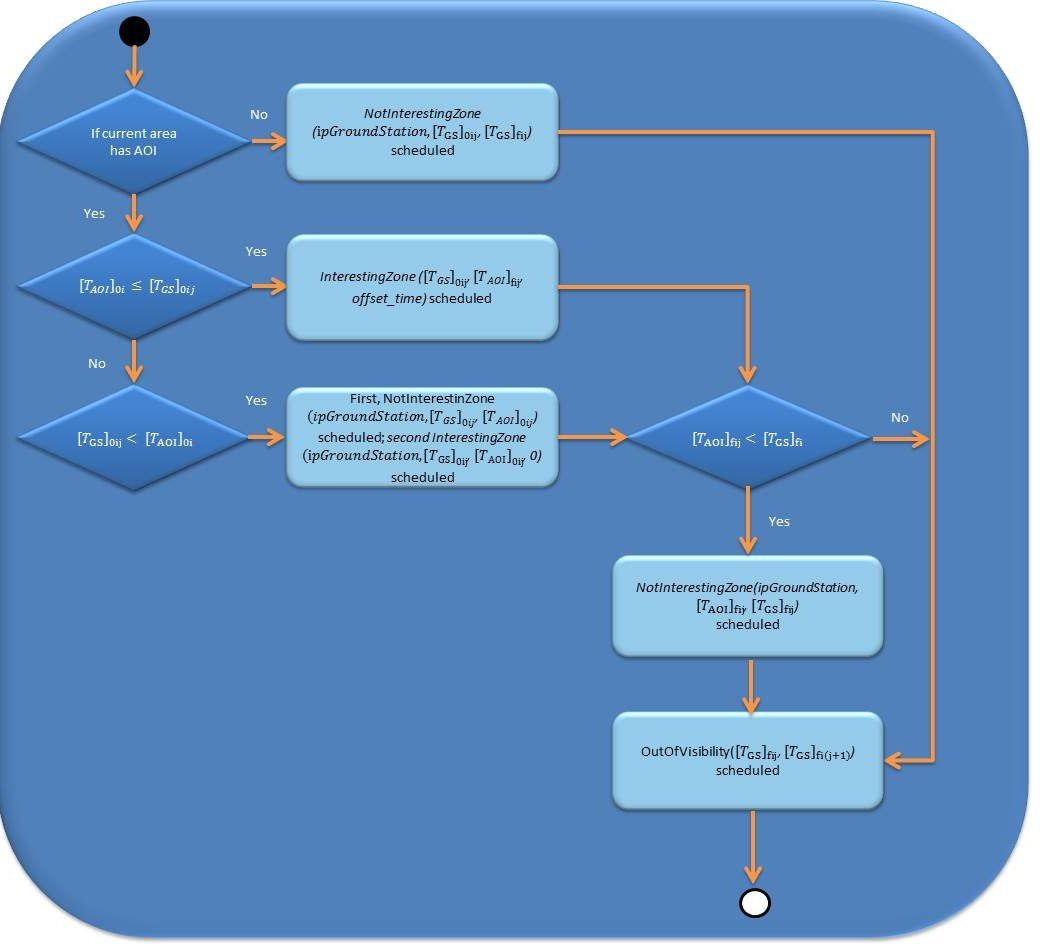
\includegraphics[width=1\textwidth]{spaceSystemSimulator/sheduling-process.jpg}
\caption{Sheduling Process on the Satellite Simulator}
\label{fig:sss-sheduling-process}
\end{center}
\end{figure}


The activity diagram in \emph{UML} format of the \emph{Satellite Simulator} is
depicted in Figure~\ref{fig:sss-satellite-activity}.

\begin{figure}[!h]
\begin{center}
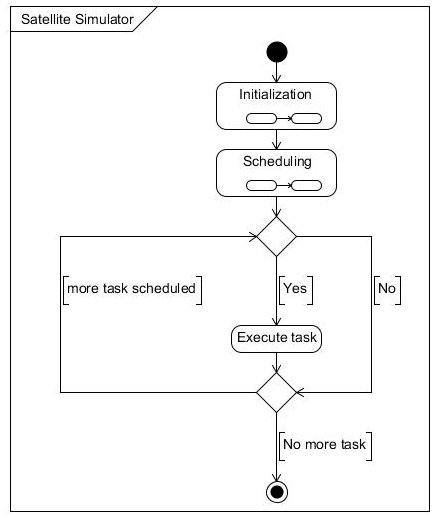
\includegraphics[width=0.6\textwidth]{spaceSystemSimulator/sat-simulator-activity.jpg}
\caption{Satellite Simulator Activity Diagram}
\label{fig:sss-satellite-activity}
\end{center}
\end{figure}

\paragraph{Satellite Simulator Implementation}
\label{par:sat-simulator-implementation}~\\

The implementation was done in Python 2.7. The python's libraries needed to
implement the software are listed in Table~\ref{table:sss-satellite-libraries}.



\begin{table}[h]
  \centering
  {\small
  


\begin{tabular}{p{.2\textwidth}p{.2\textwidth}}
  \tabheadformat
  \tabhead{Python Library}   &
  \tabhead{Function}\\
\hline
\textit{Sys}         & System library \\
\hline
\textit{OS}         & Operative system interactions supply \\
\hline
\textit{Sched}         & Library that allow the Satellite Simulator to schedule the task along  the time \\
\hline
\textit{Time}         & For managing the time \\
\hline
\textit{Socket}         & Library for creating and establishing connections with other host \\
\hline
\textit{Pdb}         &  Used for debugging the software\\
\hline
\textit{Logging}         &Log      \\
\hline
\end{tabular}


% Local variables:
%   coding: utf-8
%   ispell-local-dictionary: "castellano8"
%   TeX-master: "main.tex"
% End:

  }
  \caption{Satellite Simulator's Python Libraries}
  \label{table:sss-satellite-libraries}
\end{table}

When we installed Python, all the libraries were installed with the exception of ``MySQLdb'', which was manually installed.

Furthermore, STK provided the time in the next formats:
\begin{itemize}
\item \emph{UTCG format:} Universal Time Coordinated in Gregorian format.
\item \emph{Format in seconds:} total of seconds
\end{itemize}
They are the absolute time from the beginning of the constellation simulation in
the STK software. In the data base, the stored times are implemented in
seconds. However to simulate a scenario in real time is too long. It can be
shortened by computing a relative time $(T_r)$:
\begin{equation}\label{eq:TR}
	T_r=T/n
\end{equation}

where $T$ is the absolute time and $n$ a factor that scales the absolute time to
reduce the execution time of the experiment. In preliminary simulations we used
$n=10$, although during the experiment execution stage this will be evaluated
and probably changed. The Table~\ref{table:sss-scenario-relative-time} shows the absolute times and relative times for each scenario duration.


\begin{table}[h]
  \centering
  {\small
  


\begin{tabular}{p{.2\textwidth}p{.2\textwidth}p{.2\textwidth}}
  \tabheadformat
  \tabhead{Scenario}   &
  \tabhead{Absolute Time}&\tabhead{Relative Time}\\
\tabheadformat
& \tabhead{$(T_0,T_f)$} & \tabhead{$(T_{r0}, T_{rf})$}\\
\tabheadformat
&\tabhead{(Seconds)}& \tabhead{(Seconds)}\\
\hline
\textit{Scenario 1: Emergencies – Lorca Earthquake (Spain)}         & (63638, 63661)& (6363.8, 6366.1)\\
\hline
\textit{Scenario 2: Infrastructure monitoring. Affection in railway infrastructures by sand movement in desert areas (Spain)}         & (54060, 54753) & (5406.0, 5475.3)\\
\hline
\textit{Scenario 3: Land Management – South West of England}         & (62480, 63865)& (6248.0, 6386.5) \\
\hline
\textit{Scenario 4: Precision Agriculture – Argentina}         & (78461, 84999) & (7846.1, 8499.9) \\
\hline
\textit{Scenario 5: Basemaps – Worldwide}         & (0, 86400) & (0, 8640.0)\\
\hline
\end{tabular}


% Local variables:
%   coding: utf-8
%   ispell-local-dictionary: "castellano8"
%   TeX-master: "main.tex"
% End:

  }
  \caption{Scenarios relative times}
  \label{table:sss-scenario-relative-time}
\end{table}


\paragraph{Execution}~\\
\label{par:sat-simulator-execution}
To execute the \emph{Satellite Simulator Software} the following dependencies are
required:
\begin{itemize}
\item Operative System based in \emph{GNU Debian}.
\item Python v.2.7
\item Python packages (Table~\ref{table:sss-satellite-libraries}).
\item Ethernet interface for the network connection.
\item Connectivity with the data base located in \bonfire through the network.
\end{itemize}
The \satss software is developed in a multiplatform language, but it is restricted to be executed in \emph{UNIX} operative systems because there are many dependencies with some packages and the file system.

The execution of the satellite software has to be done as \emph{super-user} in
\emph{UNIX}. It is executed with the following command line:
\begin{itemize}
\item[>] python~satellite.py~<IDSAT>~<SCENARIO>~<DBHOST>~[LOGLEVEL]
\end{itemize}

where:
\begin{itemize}
\item \emph{IDSAT} is the satellite identity. This value must be an integer.
\item \emph{SCENARIO} is the scenario number to simulate. Must be an integer.
\item \emph{DBHOST} is the host where the data base is located. Must be a hostname or an \emph{IP address}.
\item \emph{LOGLEVEL} is the level of log that the software will show. The values can be: INFO, DEBUG. This parameter is optative. By default its value is INFO.
\end{itemize}

\subsection{Ground Station System Simulator}

In this section, the implementation and the architecture of the \emph{Ground Station Simulator} is described. The \gsss reproduces the behaviour of the set of 12 ground stations by replicating 12 times a \emph{Ground Station Simulator} that renders individual ground stations behaviour.

The \gsss is a manager that executes 12 \emph{Ground Station Simulators}. The
\gsss requires the scenario number and the \emph{IP address} of the database as
an input and executes the \emph{Ground Station  Simulators} by providing them
the specific identity of the ground station \emph{(idGroundStation)}, number of
the scenario \emph{(S)} and \emph{IP address} of the distributed database
\emph{(ipDatabase)}.

\subsubsection{Ground Station Simulator}

The functions of the ground stations are the following:
\begin{itemize}
\item To receive the images sent by the satellites.
\item To create the files with the raw images that the \emph{Orchestrator} will
  download for processing and publishing in the \emph{Archive and Catalogue} subsystem.
\end{itemize}

The \emph{Ground Station Simulator} software is common for all the ground stations, but it is parameterized to define each of them, similarly to the \emph{Satellite Simulator}.

The \emph{Ground Station Simulator} is constituted by the following components:
\begin{enumerate}
\item \emph{Initialization Module:} This module obtains the following parameters
  and   initializes the \emph{Ground Station Simulator}:
\begin{itemize}
\item \emph{S:} the number of the scenario to simulate.
\item \emph{idGroundStation:} identification number of the ground station (1 to 12).
\item \emph{ipDatabase:} \emph{IP address} of the database.
\end{itemize}

Once obtained the previous parameters, the \emph{Initialization Module} connects
with the database and fetches the name of the ground station. Also, a query to
update the \emph{IP address} and port of the \emph{Ground Station Simulator} server is sent to the database.
\item \emph{Ground Station Dynamics Module:} This module represents the dynamics and associated parameters of the ground station. It requires \emph{S}, \emph{ipDatabase} and \emph{idGroundStation}.
\end{enumerate}
Figure~\ref{fig:sss-ground-station-architecture} shows the relation between the previous modules.

\begin{figure}[!h]
\begin{center}
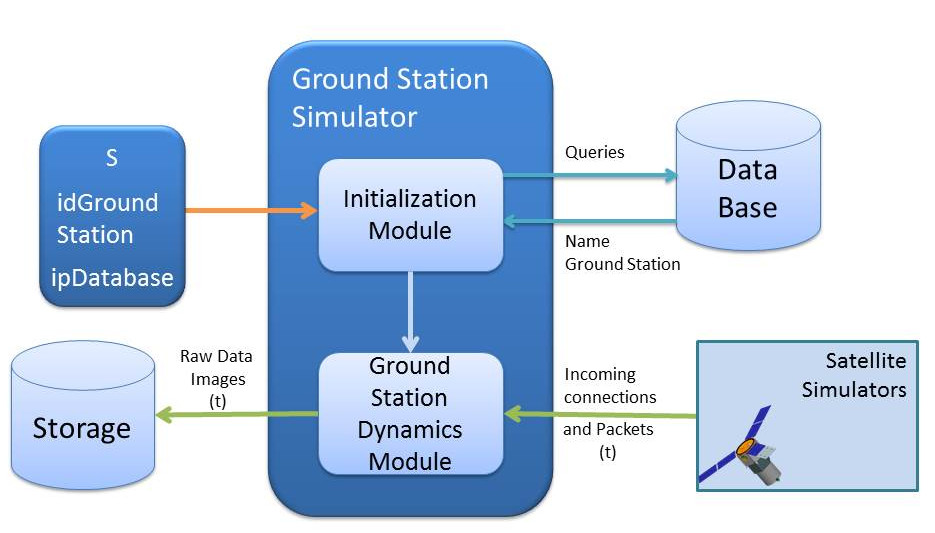
\includegraphics[width=0.7\textwidth]{spaceSystemSimulator/ground-station-architecture.jpg}
\caption{Ground Station Simulator Architecture}
\label{fig:sss-ground-station-architecture}
\end{center}
\end{figure}

\subsubsection{Ground Station Simulator Workflow}

The \emph{Ground Station Simulator} starts the execution following these steps:
\begin{enumerate}
\item The \emph{Initialization Module} obtains \emph{S}, \emph{idGroundStation} and \emph{ipDatabase}.
\item Then, the \emph{Initialization Module} queries on the database for the
  name of the ground station and for updating the \emph{IP address} and
  \emph{port} of the \emph{Ground Station Simulator}.
\item The \emph{Ground Station Dynamics Module} starts:
\begin{itemize}
\item A network socket\footnote{Network socket is an endpoint of an inter-process communication flow across a computer network. Most of the communications between computers are based on the Internet Protocol using network sockets.}  is created for listening input connections from \emph{Satellite Simulators}.
\item Every time a satellite enters into the visibility cone of the ground station a connection between a \emph{Satellite Simulator} and the \emph{Ground Station Simulator} is created. Note that if several satellites are in the same visibility cone, the \emph{Ground Station Simulator} opens a connection for each \emph{Satellite Simulator}, and that the \emph{Ground Station Simulator} can listen to new connections if new satellites enter into the visibility cone.
\item The \emph{Ground Station Simulator} creates a new process to keep the previous connection or connections (if there are more than one satellite in the visibility cone) open.
\item The new process or processes receive the packets sent by the \emph{Satellite Simulators}.
\item Once the transmission between the \emph{Satellite Simulators} and the \emph{Ground Station Simulator} finished the connections are closed.
\item Then the received packets are counted and classified by type (see Section~\ref{subpar:shedule-process}):
\begin{itemize}
\item \emph{Packet ``U'':} $98.6~Mb$ are added to the \emph{AOI} buffer and $64.1~Mb$ are added to the \emph{non AOI} buffer in the \emph{Ground Station Simulator}.
\item \emph{Packet ``I'':} $160~Mb$ are added to the \emph{non AOI} buffer in the \emph{Ground Station Simulator}.
\item \emph{Packet ``B'':} $160~Mb$ are added to the \emph{AOI} buffer in the
  \emph{Ground   Station Simulator}.
\end{itemize}
After classifying the packets, the new processes finish.
\item The \emph{AOI} images and \emph{non AOI} images are created in the \emph{Ground Station  Simulator}.
\end{itemize}
\item The \emph{Ground Station Simulator} server ends when it receives the \emph{SIGINT} signal.
\end{enumerate}

Figure~\ref{fig:sss-ground-station-workflow} shows the process explained above. The diagram also shows the interactions with the other subsystems (see Figure~\ref{fig:sss-ground-station-architecture}). Figure~\ref{fig:sss-ground-station-workflow} shows the inputs for the \emph{Ground Station Simulator} and the outputs after its execution. These outputs are the Raw Images in time created and a log file that contains the information about the execution.

\begin{figure}[!h]
\begin{center}
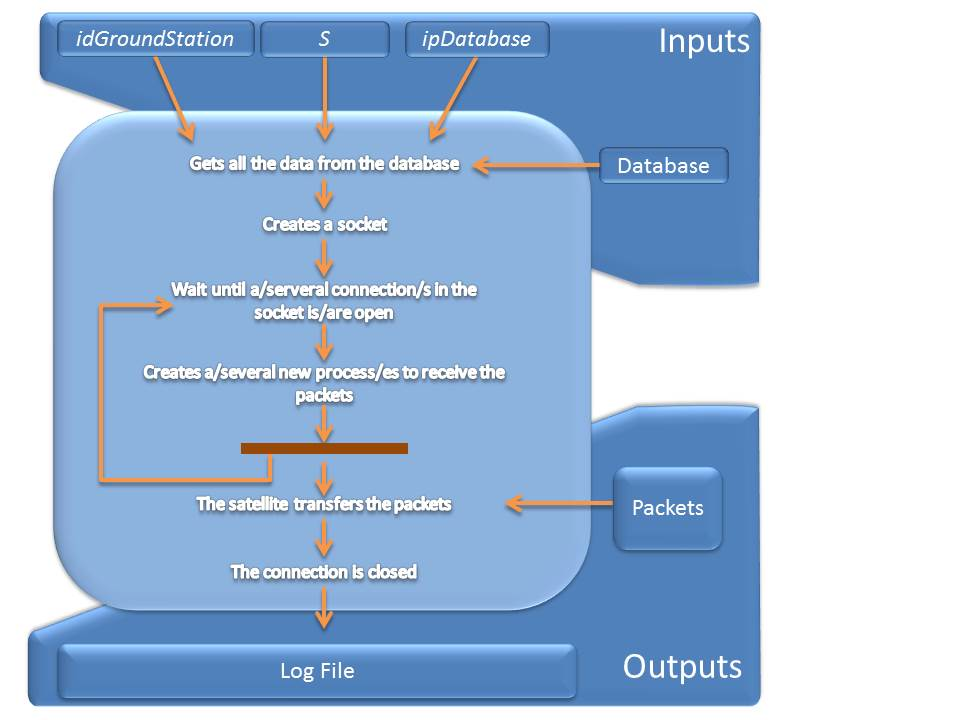
\includegraphics[width=0.85\textwidth]{spaceSystemSimulator/ground-station-workflow.jpg}
\caption{Ground Station Simulator Workflow}
\label{fig:sss-ground-station-workflow}
\end{center}
\end{figure}

The activity diagram of the Ground Station Simulator in UML format  is depicted
in Figure~\ref{fig:sss-ground-station-activity}.

\begin{figure}[!h]
\begin{center}
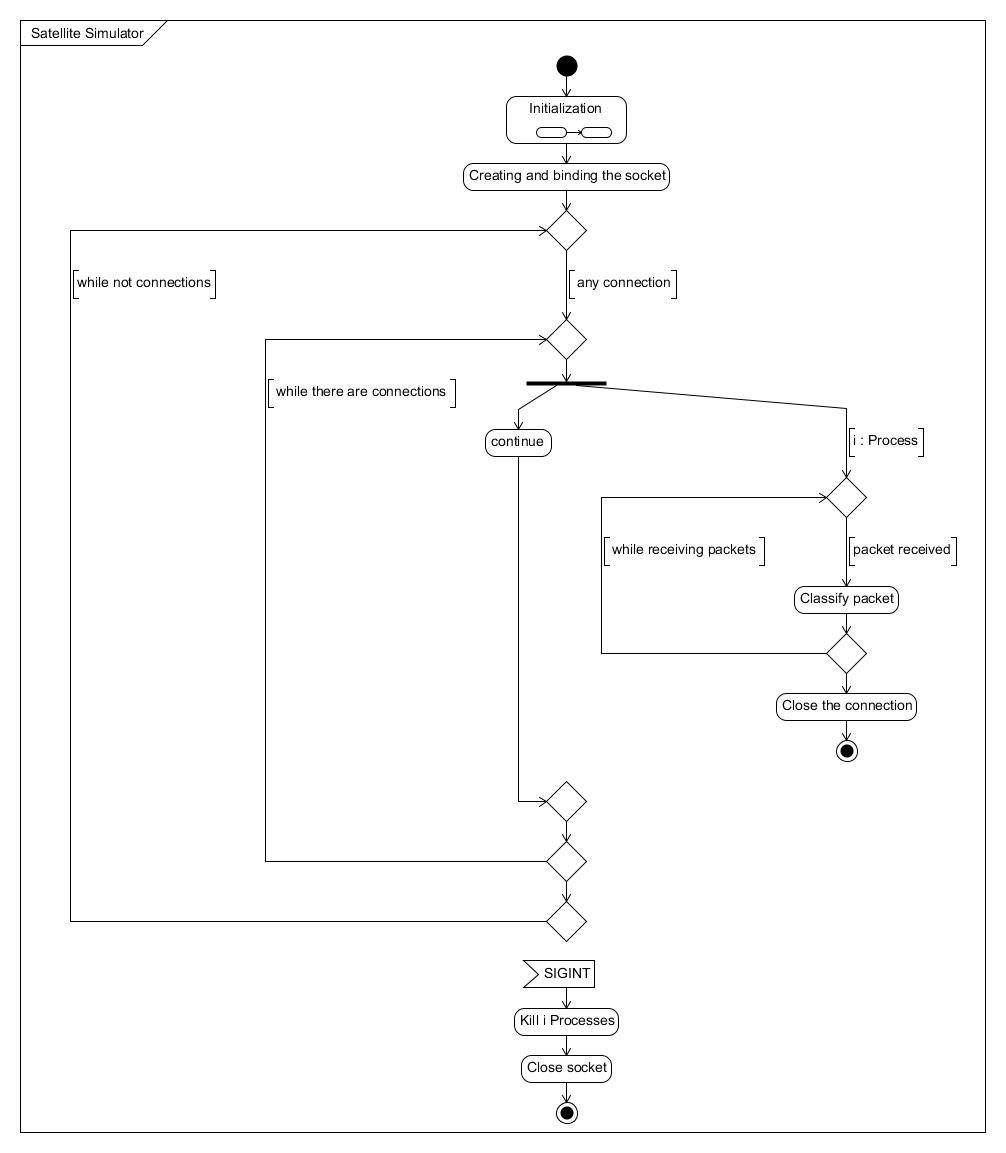
\includegraphics[width=0.9\textwidth]{spaceSystemSimulator/ground-station-activity.jpg}
\caption{Ground Station Simulator Activity Diagram}
\label{fig:sss-ground-station-activity}
\end{center}
\end{figure}

\paragraph{Implementation}\label{par:sss-ground-implementation}~\\
The implementation was done in Python 2.7, using the libraries described in
Table~\ref{table:sss-ground-libraries}.

\begin{table}[h]
  \centering
  {\small
  


\begin{tabular}{p{.2\textwidth}p{.2\textwidth}}
  \tabheadformat
  \tabhead{Python Library}   &
  \tabhead{Function}\\
\hline
\textit{Sys}         & System library \\
\hline
\textit{OS}         & Operative system interactions supply \\
\hline
\textit{Sched}         & Library that allow the Satellite Simulator to schedule the task along  the time \\
\hline
\textit{Time}         & For managing the time \\
\hline
\textit{Socket}         & Library for creating and establishing connections with other host \\
\hline
\textit{Pdb}         &  Used for debugging the software\\
\hline
\textit{Logging}         &Log      \\
\hline
\end{tabular}


% Local variables:
%   coding: utf-8
%   ispell-local-dictionary: "castellano8"
%   TeX-master: "main.tex"
% End:

  }
  \caption{Ground Station Simulator Python Libraries}
  \label{table:sss-ground-libraries}
\end{table}

\paragraph{Execution}\label{par:sss-ground-execution}~\\
To execute the Ground Station Simulator Software the following dependencies are
required:
\begin{itemize}
\item Operative System based in \emph{GNU Debian}.
\item Python v.7.
\item Python packages: (shows in Table~\ref{table:sss-ground-libraries}).
\item Ethernet interface for the network connection.
\item Connectivity with the data base located in \bonfire through the network.
\end{itemize}

The \emph{Ground Station Simulator} is developed in a multiplatform language, but it is restricted to be executed in \emph{UNIX} operative systems because there are many dependencies with some packets and the file system.

The software also needs to know the \emph{IP addresses} assigned to its Ethernet interface. If this interface is not connected, the software looks for the WLAN0 interface. This information is accomplished from the \emph{UNIX} file ``/etc/hosts''.

The execution of the satellite software must be done as sudo user as follows:
\begin{itemize}
\item[>]python~groundstation.py~<IDSAT>~<SCENARIO>~<DBHOST>~[LOGLEVEL]
\end{itemize}

where:
\begin{itemize}
\item \emph{IDSAT} is the ground station identity. This value must be an integer.
\item \emph{SCENARIO} is the scenario to simulate. It must be an integer.
\item \emph{DBHOST} is the host where the data base is located. It must be a hostname or an \emph{IP address}.
\item \emph{LOGLEVEL} is the level of log that the software will show. The
  values can be: INFO, DEBUG. This parameter is optative. Its value is INFO by default.
\end{itemize}
